\chapter{Kaons Interactions in Argon: Cross Section}\label{ch:Interactions}
\section{Literature Review}

%the prediction of the total hadronic interaction cross section ($\pi^{\pm}$, Ar) for thin-target simulations from two Monte Carlo generators (Geant 4.10.1 with Bertini Cascade model~\cite{geant4, g4bert} and Genie v2.8.2 with intranuke-hA model). The thick target simulation used a simple stand-alone Geant4 simulation  (i.e., no other detector features were taken into account except the geometry of the thin slices in the LAr volume). Fig.~\ref{fig:xsplot} shows the resulting total ${\pi^-}$ cross section extracted by the sliced TPC technique; it agrees well with the Geant 4 thin-target cross section. The Genie thin-target cross section for $^{40}$Ar shown in this figure is significantly different than that of Geant at low kinetic energies due to the fact that Geant4 models are tuned on $^{12}$C while Genie ones are tuned on a much heavier $^{56}$Fe target. The extrapolated cross section predicted for $^{40}$Ar can be then very different, especially in the resonance region where the model is strongly target-dependent from one generator to another.
 
%The comparison of the Geant4 thin- and thick-target cross section results demonstrates the power of the "sliced TPC" method for the measurement of the ($\pi^{\pm}$, Ar) cross section in LArIAT TPC geometry. 


%Having validated the ``Sliced TPC'' technique and shown that the this technique recovers the simulated cross-section, we now move to performing this measurement utilizing the complete LArIAT simulation within the LArSoft \cite{} based simulation.  Furthermore, we move from utilizing particle level MC-truth information to performing fully automated reconstruction of the charged hadron events within the LArTPC. 


%Since the kaon cross section in argon has never been measured before, the Geant4 Monte Carlo tunes kaon transportation in argon by extrapolation from lighter and heavier nuclei. As shown in the previous section,  kaon data on carbon are available and  can be used as a metric to evaluate the Geant4 prediction performances.  Figure \ref{fig:TrueCarbon} shows the total hadronic cross section for carbon implemented in Geant4 10.01.p3 overlaid with the Bugg and Friedman data. Unfortunately, the current version of Geant4 does not reproduce the data for carbon closely. On one hand, this evidence makes us even more wary when using the Monte Carlo in simulating the kaon-argon interactions. On the other, it further highlights the importance of kaon measurements.

\section{How to Measure Hadron Cross Section in LArIAT}\label{ch:methodology}
We use both the LArIAT  beamline detectors and the LArTPC information in order to measure hadronic cross sections in argon. Albeit with small differences, both the  $\pi^{-}$-Ar and K$^{+}$-Ar total hadronic cross section measurements rely on the same procedure described in details in the following paragraphs: we select the particle of interest using a combination of beamline detectors and TPC information (paragraph \ref{ch:ParticleSelectionMethod}), we perform a handshake between the beamline information and the TPC tracking to assure we are selecting the right TPC track (paragraph \ref{ch:WC2TPCMatchMethod}), and we apply the ``thin slice" method to get to the final result (paragraph \ref{ch:ThinSliceMethod}).
\subsection{Particle Selection}\label{ch:ParticleSelectionMethod}
\subsection{Wire Chamber to TPC Match}\label{ch:WC2TPCMatchMethod}
After an event passes the selection described in the previous paragraph, we need to identify the track inside the TPC corresponding to the particle which triggered the beamline detectors, a procedure we refer to as ``WC to TPC match". In general, the tracking algorithm will reconstruct more than one track in the event, partially due to the fact that hadrons interact in the chamber, as shown in figure , and partially because of pile up events where the beam of charge particle is too intense compared to the drift time, as shown in figure. 
\textcolor{red}{EVENT DISPLAYS}



\subsection{The Thin Slice Method}\label{ch:ThinSliceMethod}
\subsubsection{Cross Sections on Thin Target}
Cross section measurements on a thin target have been the bread and butter of nuclear and particle {Iexperimentalists since the Rutherford experiments \textcolor{red}{NEED CITATION}. At their core, this type of experiments consists in shooting a beam of particles with a known flux on a thin target and recording the outgoing flux. 


In general, the target is not a single particle, but rather a slab of material containing many diffusion centers. The so-called  ``thin target" approximation assumes that the target centers are uniformly distributed in the material and that the target is thin compared to the interaction length so that no center of interaction sits in front of another. In this approximation, the ratio between the number of particles interacting in the target $N_{Interacting}$ and number of incident particles $N_{Incident}$ determines the interaction probability $P_{Interacting}$, which is the complementary to one of the survival probability $P_{Survival}$. 
Equation \ref{eq:thinTargetXS} 
\begin{equation}
P_{Survival} = 1- P_{Interacting} = 1 - \frac{N_{Interacting}}{N_{Incident}} = e^{-\sigma_{TOT} n \delta X}
\label{eq:thinTargetXS}
\end{equation}
describes the probability for a particle to survive the thin target. This formula relates the total cross section $\sigma_{TOT}$, the density of the target centers  $n$  and  the thickness of the target  along the incident hadron direction $\delta X$, to the interaction probability\footnote{The scattering center density in the target, {\emph{n}},  relates to the argon density $\rho$, the Avogadro number  $ N_{A} $ and the argon molar mass $m_A$ as $n=\frac{\rho N_{A} }{m_A}$.}. If the target is thin compared to the interaction length of the process considered, we can Taylor expand the exponential function in equation \ref{eq:thinTargetXS} and find a simple proportionality relationship between the number of incident and interacting particles, and the cross section, as shown in equation \ref{eq:thinTargetXSTaylor}:
\begin{equation}
1 - \frac{N_{Interacting}}{N_{Incident}} =  1 -\sigma_{TOT} n \delta X + O(\delta X^2).
\label{eq:thinTargetXSTaylor}
\end{equation}

Solving for the cross section, we find:
\begin{equation}
 \sigma_{TOT}  = \frac{1}{n \delta X}\frac{N_{Interacting}}{N_{Incident}}.
\label{eq:thinTargetXSSolved}
\end{equation}

\subsubsection{Not-so-Thin Target: Slicing the Argon}
The LArIAT TPC, with its 90 cm of length, is not a thin target. \textcolor{red}{Find expected interaction length for hadrons and kaons}. However, the fine-grained tracking of the LArIAT LArTPC allows us to treat the argon volume as a sequence of many adjacent thin targets. 

As described in section \ref{sec:experimentDescription}, LArIAT wire planes count 240 wires each. The wires are oriented at +/- $60^{\circ}$ from the vertical direction at 4 mm spacing, while the beam direction is oriented 3 degrees off the $z$ axis in the $XZ$ plane. \textcolor{red}{review this math} The wires collect signals proportional to the energy loss of the hadron along its path in a  $\delta${\emph{X}} = 4 mm/sin($60^{\circ}$) $\approx$ 4.7~mm slab of liquid argon. Thus, one can think to slice the TPC into many thin targets of $\delta${\emph{X}} = 4.7~mm thickness along the direction of the incident particle. 

Considering each slice {\emph{j}}  a ``thin target",  we can apply the cross section calculation from Eq.~\ref{eq:thinTargetXSSolved} iteratively, evaluating the kinetic energy of the hadron as it enters each slice, $E_{j}^{kin}$.  For each WC-to-TPC matched particle, the energy of the hadron entering the TPC is known thanks to the momentum and mass determination by the tertiary beamline, 

\begin{equation}
 E^{kin}_{Front Face}  = \sqrt{p^2_{Beam} - m^2_{Beam}} - E_{loss},
\label{eq:enFF}
\end{equation}
where $E_{loss}$ is a correction for the energy loss in the dead material between the beamline and the TPC front face (more on \ref{sec:Eloss}). The  energy of the hadron at the each slab is determined by subtracting the energy released by the particle in the previous slabs. For example, at the $j^{th}$ point of a track, the kinetic energy will be

\begin{equation}
 E_{j}^{kin} =  E^{kin}_{Front Face} - \sum_{i < j} \Delta E_i,
\label{eq:KEj}
\end{equation}
where $\Delta E_i$ is the energy deposited at each argon slice before the $j^{th}$ point as measured by the calorimetry associated with the tracking.


If the particle enters a slice, it contributes to $N_{Incident}( E^{kin})$ in the energy bin corresponding to its kinetic energy in that slice. If it interacts in the slice, it then also contributes to $N_{Interacting}(E^{kin})$ in the appropriate energy bin. The cross section as a function of kinetic energy, $\sigma_{TOT}( E^{kin})$ will then be proportional to the ratio $\frac{N_{Interacting}( E^{kin})}{N_{Incident}( E^{kin})}$ .


The statistical uncertainty for each energy bin is calculated by error propagation from the statistical  uncertainty on $N_{Incident}$ and $N_{Interacting}$. 
Since the number of incident hadrons in each energy bin is given by a simple counting, we assume that $N_{Incident}$ is distributed as a poissonian with mean and $\sigma^2$ equal to $N_{Incident}$ in each bin.  
On the other hand, $N_{Interacting}$ follows a binomial distribution: a particle in a given energy bin might or might not interact.  The square of the variance for the binomial is given by  
\begin{equation}
\sigma^2 = \mathcal{N}P_{Interacting}(1-P_{Interacting});
\label{eq:binVar}
\end{equation}

since the interaction probability $P_{Interacting}$ is $\frac{ N_{Interacting}}{N_{Incident}}$ and the number of tries $\mathcal{N}$ is $N_{Incident}$, equation \ref{eq:binVar} translates into
\begin{equation}
\sigma^2 = N_{Incident}\frac{ N_{Interacting}}{N_{Incident}} (1-\frac{ N_{Interacting}}{N_{Incident}}) = N_{Interacting}(1-\frac{ N_{Interacting}}{N_{Incident}}).
\end{equation}

$N_{Incident}$ and $N_{Interacting}$ are not independent.
The uncertainty on the cross section is thus calculated as 
\begin{equation}
\delta\sigma_{tot}(E) = \sigma_{tot}(E) \Big(\frac{\delta N_{Interacting}}{N_{Interacting}}+\frac{\delta N_{Incident}}{N_{Incident}}\Big) 
\end{equation}
where:
\begin{eqnarray}
\delta N_{Incident} = \sqrt[]{N_{Incident}} \\
\delta N_{Interacting} = \sqrt[]{N_{Interacting}(1-\frac{ N_{Interacting}}{N_{Incident}})}.
\end{eqnarray}


%%%%%%%%%%%%%%%%%%%%%%%%%%%%%%%%%%%%%%%%%%%%%%%%



\subsection{Procedure testing with truth quantities}
The $\pi^{-}$-Ar and K$^{+}$-Ar total hadronic cross section implemented in Geant4 can be used as a tool to validate the measurement methodology.  We describe here a closure test done on Monte Carlo to prove that the methodology of slicing the TPC retrieves the underlying cross section distribution implemented in Geant4 within the statistical error. %under the working assumption of perfect reconstruction.

For pions in the considered energy range, \textcolor{red}{the Geant4 inelastic model adopted to is ``BertiniCascade", while the elastic model ``hElasticLHEP".}
For kaons, the Geant4 inelastic model adopted to is ``BertiniCascade", while the elastic model ``hElasticLHEP".  


For the validation test, we fire about 390000 pions and 140000 kaons inside the LArIAT TPC active volume using the DDMC (see sec \ref{ch:DDMC}). We apply  the thin-sliced method on using true quantities to calculate the hadron kinetic energy at each slab in order to decouple reconstruction effects to eventual issues with the methodology.  For each slab of 4.7 mm length on the path of the hadron, we integrate the true energy deposition as given by the Geant4 transportation model. Then, we recursively subtracted it from the hadron kinetic energy at the TPC front face to evaluate the kinetic energy at each slab until the true interaction point is reached. Doing so, we obtain the true interacting and incident distributions for the considered hadron and we obtain the true MC cross section as a function of the hadron true kinetic energy. 

Figure \ref{fig:TrueMCXS} shows the total hadronic cross section for argon implemented in Geant4 10.01.p3 (solid lines) overlaid with the true MC cross section as obtained with the sliced TPC method (markers) for pions on the left and kaons on the right; the total cross section is shown in green,  the elastic cross section in blue and the inelastic cross section in red.  The nice agreement with the Geant4 distribution and the cross section  obtained with the sliced TPC method gives us confidence in the  validity of the methodology. 
        
%\begin{comment}     
\begin{figure}
%\captionsetup{justification=raggedright}  
\begin{minipage}[b]{.53\textwidth}  
  \centering  
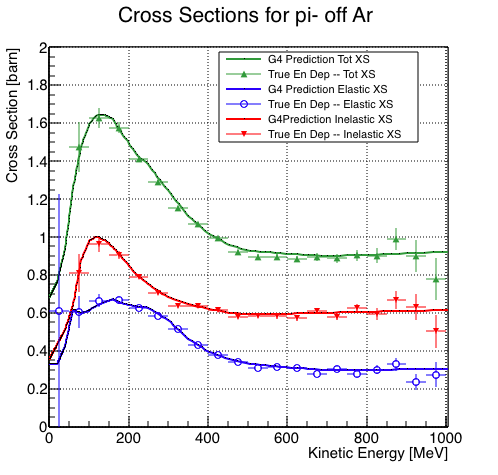
\includegraphics[width=3in]{Chapter-4/Images/PionTrueXS.png}
\end{minipage}%  
\begin{minipage}[b]{0.53\textwidth}  
  \centering  
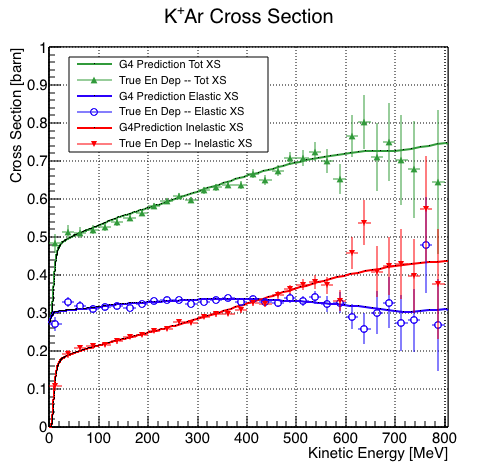
\includegraphics[width=3in]{Chapter-4/Images/KaonTrueXS.png}
\end{minipage}
\label{fig:TrueMCXS}
\caption{Hadronic cross sections for $\pi^-$-Ar (left) and K$^+$-Ar (right) implemented in Geant4 10.01.p3 (solid lines) overlaid the true MC cross section as obtained with the sliced TPC method (markers). The total cross section is shown in green,  the elastic cross section in blue and the inelastic cross section in red.}
%\par
%\begin{minipage}[t]{.53\textwidth}
%\caption{total hadronic cross section for carbon implemented in Geant4  10.01.p3  with overlaid with the Bugg %and Frideman data.}
%\label{fig:TrueCarbon}
%\end{minipage}%
%\begin{minipage}[t]{.5\textwidth}  
%\caption{Hadronic cross sections for argon implemented in Geant4 10.01.p3 (solid lines) overlaid the true MC cross section as obtained with the sliced TPC method (markers). The total cross section is shown in green,  the elastic cross section in blue and the inelastic cross section in red.}
%\label{fig:TrueArgon}
%\end{minipage}  
\end{figure}
%\end{comment}


\subsection{Uncertainty budget}
Measuring an hadronic cross section  in LArIAT translates into counting how many hadrons impinged on a slab of argon at a given energy and how many of those hadrons interacted at said energy. So, the key questions here are:
\begin{itemize}
\item[]a) how well do we know the kinetic energy at each point of the tracking? %(Incident Kinetic Energy bins)
\item[]b) how well do we know when the tracking stops? %(Interacting Kinetic Energy bin)
\item[]c) are there any systematic shifts?
\end{itemize}

In order to answer this question, will discuss first a simple scenario  were our beam is 100\% made of pions which arrive as primaries in the TPC (no decay in the beam and no inelastic interaction before the TPC front face). We will then add a layer of complexity by discussing how we handle beamline contamination.
\subsubsection{Pure beam of pions}
\subsubsection{Handling beamline contamination}
What is the beamline contamination? We define beamline contamination every TPC track matched to the WC track which is not a primary pion. There are 4 different types of beamline contaminations:
\begin{itemize}
\item[]1) electrons,
\item[]2) muons,
\item[]3) secondary pions,
\item[]4) matched pile up events.
\end{itemize}
So, how do we handle this contamination?
The first step is understanding what percentage of events used in the data cross section calculation is not a primary pion. 

The number of electrons and muons in the pion sample is estimated via the beamline MC. We simulate the beamline composition for each of the magnet settings present on data (-60A and -100A). 
and we weight for the number of events which pass the mass cut in both the configurations. 
For each beamline 

We estimate the matched pile up events to be a negligible fraction, because of the definition of the WC2TPC match: we deem the probability of a single match\footnote{ Events with multiple matches are rejected.} with a pile up event in the absence of a real particle  within a four centimeter radius from the WC track projection extremely small.

